% !TEX root = tutor-1-12-4.tex
% Edit tasks in task-1-12-4.tex.
\def\TutorEdition{1}
\expandafter\def\csname TutorSourceB0907A\endcsname{\href{https://ege.fipi.ru/bank/questions.php?search=1\&proj=BA1F39653304A5B041B656915DC36B38\&qid=B0907A}{Источник: B0907A}}
\expandafter\def\csname TutorSource0BA328\endcsname{\href{https://ege.fipi.ru/bank/questions.php?search=1\&proj=BA1F39653304A5B041B656915DC36B38\&qid=0BA328}{Источник: 0BA328}}
\expandafter\def\csname TutorSource26733\endcsname{\href{https://phys-ege.sdamgia.ru/problem?id=26733}{Источник: Решу ЕГЭ, №26733}}
\expandafter\def\csname TutorSource25401\endcsname{\href{https://phys-ege.sdamgia.ru/problem?id=25401}{Источник: Решу ЕГЭ, №25401}}
\expandafter\def\csname TutorSource25744\endcsname{\href{https://phys-ege.sdamgia.ru/problem?id=25744}{Источник: Решу ЕГЭ, №25744}}
\expandafter\def\csname TutorSource51478\endcsname{\href{https://phys-ege.sdamgia.ru/problem?id=51478}{Источник: Решу ЕГЭ, №51478}}
% !TEX root = task-1-12-4.tex
% Editable task bank. Append new BankTask blocks at the end of the document.
\documentclass[12pt,a4paper]{article}
\usepackage{physics-textbook}
\usepackage{graphicx,needspace}
\usetikzlibrary{decorations.pathmorphing}
\newif\ifShowSolutions
\ifdefined\TutorEdition
  \ShowSolutionstrue
\else
  \ShowSolutionsfalse % Change to \ShowSolutionstrue to display solutions.
\fi
\newcounter{banktask}
\newsavebox{\BankTaskBox}
\newcommand{\BankTaskContent}[3]{%
  \noindent\textbf{\thebanktask.}\quad #2\par
  \ifShowSolutions
    \Needspace{50mm}% Keep the solution heading with its opening text or diagram.
    #3\par
    \ifdefined\TutorEdition
      \ifcsname TutorSource#1\endcsname
        \nopagebreak\smallskip{\small\csname TutorSource#1\endcsname\par}%
      \fi
    \fi
  \fi
}
\newcommand{\BankTask}[3]{%
  \refstepcounter{banktask}\par\medskip
  \sbox{\BankTaskBox}{\begin{minipage}{\linewidth}%
    \BankTaskContent{#1}{#2}{#3}\end{minipage}}%
  \ifdim\dimexpr\ht\BankTaskBox+\dp\BankTaskBox\relax>\dimexpr\textheight-20mm\relax
    \Needspace{35mm}\BankTaskContent{#1}{#2}{#3}%
  \else
    \Needspace{\dimexpr\ht\BankTaskBox+\dp\BankTaskBox\relax}%
    \noindent\usebox{\BankTaskBox}\par
  \fi
  \medskip
}
\begin{document}
\BookSubsection{1.12.4}{Рычаг с грузами}


% Source B0907A: https://ege.fipi.ru/bank/questions.php?search=1&proj=BA1F39653304A5B041B656915DC36B38&qid=B0907A
\BankTask{B0907A}{
Ученик выполнял лабораторную работу по исследованию условий равновесия лёгкого рычага под действием двух сил. Полученные результаты он занёс в таблицу. Результат выразите в $\text{м}$.
\begin{center}\begin{tabular}{|c|c|c|c|}\hline
$F_1,\,\text{Н}$ & $l_1,\,\text{м}$ & $F_2,\,\text{Н}$ & $l_2,\,\text{м}$ \\\hline
$60$ & $?$ & $120$ & $0{,}2$ \\\hline
\end{tabular}\end{center}
Каково плечо $l_1$, если рычаг находится в равновесии?
}{
\smallskip\noindent\textbf{Решение от GPT}\par
Условие равновесия $F_1l_1=F_2l_2$. Тогда $l_1=120\cdot0{,}2/60=0{,}4\,\text{м}$.
}

% Source 0BA328: https://ege.fipi.ru/bank/questions.php?search=1&proj=BA1F39653304A5B041B656915DC36B38&qid=0BA328
\BankTask{0BA328}{
Момент первой силы, действующей на рычаг, равен $50\,\text{Н}\cdot\text{м}$. Какой должна быть вторая сила, чтобы рычаг находился в равновесии, если её плечо равно $0{,}5\,\text{м}$? Результат выразите в $\text{Н}$.
}{
\smallskip\noindent\textbf{Решение от GPT}\par
Для равновесия $F_2l_2=M_1$. Поэтому $F_2=50/0{,}5=100\,\text{Н}$.
}

% Source 26733: https://phys-ege.sdamgia.ru/problem?id=26733
\BankTask{26733}{
\begin{center}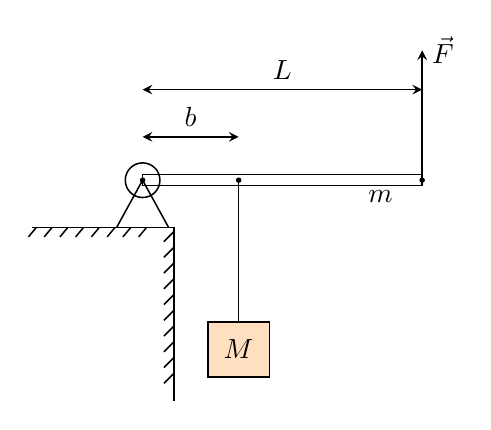
\begin{tikzpicture}[>=stealth,line width=.55pt]\draw(-1.4,-.6)--(.4,-.6)--(.4,-2.8);\foreach \x in {-1.35,-1.15,...,.25}{\draw(\x,-.6)--++(-.1,-.12);}\foreach \y in {-.65,-.85,...,-2.65}{\draw(.4,\y)--++(-.13,-.13);}\draw(-.33,-.6)--(0,0)--(.33,-.6);\draw(0,0)circle(.22);\draw(0,-.07)rectangle(3.55,.07);\fill (0,0)circle(.035) (1.22,0)circle(.035) (3.55,0)circle(.035);\draw[<->](0,1.15)--(3.55,1.15)node[midway,above]{$L$};\draw[<->](0,.55)--(1.22,.55)node[midway,above]{$b$};\draw[->](3.55,0)--(3.55,1.65)node[right]{$\vec F$};\draw(1.22,0)--(1.22,-1.8);\draw[fill=orange!25](.83,-2.5)rectangle(1.61,-1.8)node[pos=.5]{$M$};\node[below]at(3.02,0){$m$};\end{tikzpicture}\end{center}Груз массой M  =  $75\,\text{кг}$ медленно поднимают с помощью рычага, приложив вертикальную силу $\vec F$ (см. рис.). Рычаг, сделанный из однородного стержня массой m  =  $10\,\text{кг}$ и длиной L  =  $4\,\text{м}$, шарнирно закреплен. Определите модуль силы $\vec F,$ если расстояние b от оси шарнира до точки подвеса груза равно $1{,}6\,\text{м}$. Считать, что трение в шарнире отсутствует.
}{
\smallskip\noindent\textbf{Решение}\par
\begin{center}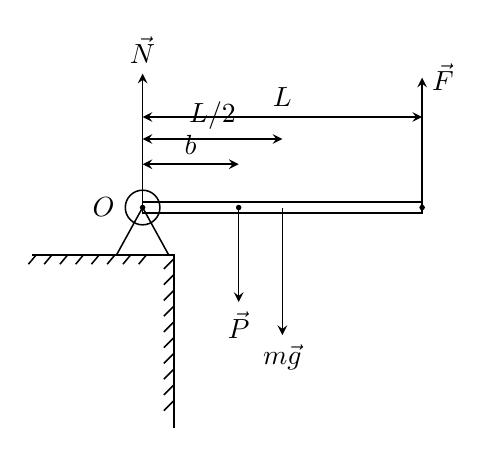
\begin{tikzpicture}[>=stealth,line width=.55pt]\draw(-1.4,-.6)--(.4,-.6)--(.4,-2.8);\foreach \x in {-1.35,-1.15,...,.25}{\draw(\x,-.6)--++(-.1,-.12);}\foreach \y in {-.65,-.85,...,-2.65}{\draw(.4,\y)--++(-.13,-.13);}\draw(-.33,-.6)--(0,0)--(.33,-.6);\draw(0,0)circle(.22);\draw(0,-.07)rectangle(3.55,.07);\fill (0,0)circle(.035) (1.22,0)circle(.035) (3.55,0)circle(.035);\draw[<->](0,1.15)--(3.55,1.15)node[midway,above]{$L$};\draw[<->](0,.55)--(1.22,.55)node[midway,above]{$b$};\draw[->](3.55,0)--(3.55,1.65)node[right]{$\vec F$};\node[left]at(-.23,0){$O$};\draw[->](0,0)--(0,1.7)node[above]{$\vec N$};\draw[<->](0,.87)--(1.775,.87)node[midway,above]{$L/2$};\draw[->](1.22,0)--(1.22,-1.2)node[below]{$\vec P$};\draw[->](1.775,0)--(1.775,-1.62)node[below]{$m\vec g$};\end{tikzpicture}\end{center}$1$.  Рассмотрим силы, действующие на рычаг (см. рис.). 
Считая, что рычаг поднимает груз медленно и равномерно, примем, исходя из третьего и второго законов Ньютона, что $|\vec{P} |=|M \vec{g}|.$
$2$.  Рассмотрим равновесие рычага относительно оси вращения  — шарнира О, указав плечи сил на рисунке. $O: Mg \cdot b + \frac{1}{2} mgL - FL=0.$
Отсюда:

\[F=Mg \cdot \frac{b}{L} + \frac{1}{2} mg=75 \cdot 10 \cdot \frac{1{,}6}{4} + \frac{1}{2} \cdot 10 \cdot 10=350\,\text{Н}.\]

Ответ: F  =  $350$ Н.
}

% Source 25401: https://phys-ege.sdamgia.ru/problem?id=25401
\BankTask{25401}{
Деревянная линейка длиной l  =  $90\,\text{см}$ выдвинута за край стола на $\frac{1}{4}$ часть своей длины. При этом она не опрокидывается, если на ее правом конце лежит груз массой не более $m_1=250\,\text{г}.$ Далее линейку выдвинули вправо за край стола на некоторое расстояние и положили на ее правый конец груз массой $m_2=125\,\text{г}.$ На какое расстояние дополнительно можно выдвинуть линейку во втором опыте, чтобы она не перевернулась?
}{
\smallskip\noindent\textbf{Решение}\par
На линейку в обоих случаях действую сила тяжести линейки, приложенная к ее середине и вес груза. Линейка находится в равновесии, поэтому можно записать правило моментов для каждого случая относительно точки опоры  — края стола. В первом случае плечи силы тяжести линейки и веса груза равны $\frac{l}{4} .$ 
Следовательно, масса линейки равна массе груза $M=m_1=250\,\text{г}.$

\begin{center}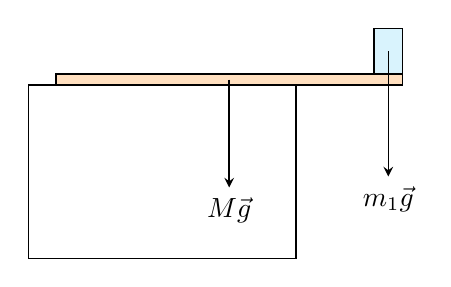
\begin{tikzpicture}[>=stealth,line width=.55pt]\draw(0,-2.2)rectangle(3.4,0);\draw[fill=orange!25](.35,0)rectangle(4.75,.14);\draw[fill=cyan!15](4.39,.14)rectangle(4.75,.72);\draw[->](4.57,.43)--(4.57,-1.16)node[below]{$m_1\vec g$};\draw[->](2.55,.07)--(2.55,-1.3)node[below]{$M\vec g$};\end{tikzpicture}\end{center}

\begin{center}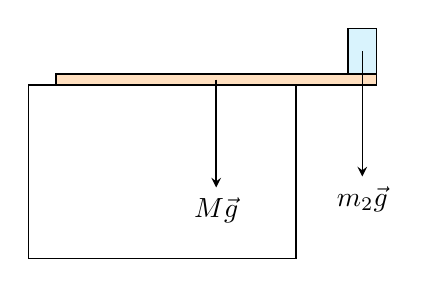
\begin{tikzpicture}[>=stealth,line width=.55pt]\draw(0,-2.2)rectangle(3.4,0);\draw[fill=orange!25](.35,0)rectangle(4.42,.14);\draw[fill=cyan!15](4.06,.14)rectangle(4.42,.72);\draw[->](4.24,.43)--(4.24,-1.16)node[below]{$m_2\vec g$};\draw[->](2.385,.07)--(2.385,-1.3)node[below]{$M\vec g$};\end{tikzpicture}\end{center}

Во втором случае плечо веса груза равно $l_2$ а плечо силы тяжести линейки $\frac{l}{2} - l_2.$
Запишем правило моментов для второго случая:

$m_2gl_2=Mg ( \frac{l}{2} - l_2 ) ,$ откуда плечо веса груза:
$l_2= \frac{Ml}{2 ( m_2 + M )} = \frac{250 \cdot 90}{2 \cdot ( 125 + 250 )} =30\,\text{см}.$

Учитывая, что в первом случае расстояние равнялось $\frac{l}{4} = \frac{90}{4} =22{,}5\,\text{см},$ линейка останется в равновесии, если ее выдвинуть на $7{,}5\,\text{см}$.

Ответ: $7{,}5\,\text{см}$.
}

% Source 25744: https://phys-ege.sdamgia.ru/problem?id=25744
\BankTask{25744}{
Два небольших шара массами $m_{1}$ = $0{,}2\,\text{кг}$ и $m_{2}$ = $0{,}3\,\text{кг}$ закреплены на концах невесомого стержня $AB$, расположенного горизонтально на опорах $C$ и $D$ (см. рис.). Расстояние между опорами l = $0{,}6\,\text{м}$, а расстояние $AC$ равно $0{,}2\,\text{м}$. Чему равна длина стержня $L$, если сила давления стержня на опору $D$ в $2$ раза больше, чем на опору $C$? Сделайте рисунок с указанием внешних сил, действующих на систему тел «стержень  — шары».
Какие законы Вы используете для описания равновесия тела? Обоснуйте их применение к данному случаю.
\begin{center}\begin{tikzpicture}[task graph,>=stealth]
\draw(.5,1)rectangle(5.5,1.15);\draw(.5,.75)circle(.25)(5.5,.75)circle(.25);
\node[above]at(.5,1.15){$A$};\node[above]at(5.5,1.15){$B$};
\node[left]at(.25,.65){$m_1$};\node[right]at(5.75,.65){$m_2$};
\draw(1.8,0)--(2,1)--(2.2,0)--cycle;\draw(4.5,0)--(4.7,1)--(4.9,0)--cycle;
\node[left]at(2,.8){$C$};\node[left]at(4.7,.8){$D$};\draw(.2,0)--(5.8,0);
\foreach \x in {.4,.6,...,5.8}{\draw(\x,0)--++(-.12,-.12);}
\end{tikzpicture}\end{center}
}{
\smallskip\noindent\textbf{Решение}\par
Обоснование. Систему отчета, связанную с Землей, будем считать инерциальной. Для данной системы отсчета можно применить законы Ньютона (в частности, третий закон).
Тело, образованное стержнем и двумя шарами, будем считать абсолютно твердыми. Движение абсолютно твердого тела представляет собой суперпозицию поступательного и вращательного движений, поэтому для него можно применить условие равновесия для поступательного движения и правило моментов. Векторная сумма всех внешних сил, действующих на тело, равна нулю, поэтому сумма моментов этих сил относительно двух любых его параллельных осей одна и таже. Для удобства ось, относительно которой будем рассматривать сумму моментов сил, проведем перпендикулярно плоскости чертежа через точку А.

Перейдем к решению. На твердое тело, образованное стержнем и двумя шарами, действуют силы тяжести $m_1\vec g$ и $m_2\vec g,$ приложенные к центрам шаров, и силы реакции опор $\vec N_1$ и $\vec N_2.$ По третьему закону Ньютона, модули сил реакции равны соответствующим модулям сил давления стержня на опоры, поэтому $N_2 = 2N_1$ (в соответствии с условием задачи).
\begin{center}\begin{tikzpicture}[task graph,>=stealth]\draw[->](-.6,-.5)--(6,-.5)node[right]{$x$};\foreach \xx in {-.6,-.44,...,5.45}{\draw(\xx,-.5)--++(.12,-.12);}\draw[->](-.6,-1.8)--(-.6,2.1)node[above]{$y$};\node[below left]at(-.6,-.5){$O$};\draw[fill=gray!10](0,.55)rectangle(5,.7);\foreach\x/\l in{0/A,5/B}{\draw[fill=gray!15](\x,.3)circle(.2);\node[above]at(\x,.85){$\l$};}\foreach\x/\l in{1.4/C,4.2/D}{\draw(\x,.55)--++(-.2,-1.05)--++(.4,0)--cycle;\node[left]at(\x,.1){$\l$};}\node[right]at(.3,.2){$m_1$};\node[right]at(5.3,.2){$m_2$};\draw[->,thick](1.4,.55)--(1.4,1.6)node[above]{$\vec N_1$};\draw[->,thick](4.2,.55)--(4.2,2)node[above]{$\vec N_2$};\draw[->,thick](0,.3)--(0,-1.4)node[right]{$m_1\vec g$};\draw[->,thick](5,.3)--(5,-1.6)node[right]{$m_2\vec g$};\end{tikzpicture}\end{center}
В инерциальной системе отсчета $Oxy$, связанной с Землей, условия равновесия твердого тела приводят к набору уравнений:

\[N_1 + N_2 - m_1g - m_2g = 0\]

  — центр масс не движется вдоль оси $Oy$.

\[N_1x + N_2 ( l + x ) - m_2gL = 0\]

  — нет вращения вокруг оси, проходящей перпендикулярно рисунку через точку $A$.
 Здесь $x = AC = 0{,}2\,\text{м}$  — плечо силы реакции $N_{1}$.
 С учетом условия $N_2 = 2N_1$ уравнения приводятся к виду:

$3N_1 = ( m_1 + m_2 ) g,$
$( 3x + 2l ) N_1 = m_2gL.$

 Поделив второе уравнение на первое, получим:

\[L \frac{m_2}{m_1 + m_2} = x + \frac{2}{3} l.\]

 Откуда:

\[L = ( 1 + \frac{m_1}{m_2} ) \cdot ( x + \frac{2}{3} l ) = ( 1 + \frac{0{,}2\,\text{кг}}{0{,}3\,\text{кг}} ) \cdot ( 0{,}2\,\text{м} + \frac{2}{3} \cdot 0{,}6\,\text{м} ) = 1\,\text{м}.\]

Ответ: $1\,\text{м}$.
}

% Source 51478: https://phys-ege.sdamgia.ru/problem?id=51478
\BankTask{51478}{
К концам невесомого рычага подвесили за невесомые нерастяжимые нити два сплошных груза массами $1{,}28\,\text{кг}$ и $0{,}32\,\text{кг}$ и привели рычаг в состояние равновесия. Затем рычаг с грузами расположили над водой так, что оба груза целиком оказались под водой. В результате для сохранения равновесия точку опоры пришлось переместить на $10\,\text{см}$. Определите первоначальное расстояние от более тяжёлого груза до точки опоры, если объёмы обоих грузов одинаковы и равны $200\,\text{см}^{3}$. Сделайте рисунок, на котором укажите силы, действующие на рычаг (для двух случаев), а также на погружённые в воду грузы.
Обоснуйте применимость законов, используемых для решения задачи.
}{
\smallskip\noindent\textbf{Решение}\par
Обоснование.
$1$.  Рассмотрим задачу в системе отсчёта, связанной с Землёй. Будем считать эту систему отсчёта инерциальной  — ИСО.
$2$.  Опишем рычаг моделью абсолютно твёрдого тела  — форма и размеры тела неизменны, расстояние между любыми двумя точками тела остаётся неизменным.
$3$.  Сумма приложенных к абсолютно твёрдому телу внешних сил равна нулю, так как тело не совершает поступательного движения.
$4$.  Сумма моментов внешних сил относительно осей, проходящих через точки O$_{1}$ и O$_{2}$ перпендикулярно плоскости рисунка, равна нулю, так как тело не совершает вращательного движения.
$5$.  Грузы на нитях могут двигаться поступательно, поэтому опишем грузы моделью материальной точки и используем второй закон Ньютона.
$6$.  Нити невесомы, поэтому натяжение нити всюду одинаково.
$7$.  Согласно третьему закону Ньютона силы, с которыми взаимодействуют грузы, нити и рычаг, равны по модулю и направлены в противоположные стороны.
\begin{center}\begin{tikzpicture}[task graph,>=stealth]\draw[fill=gray!10](0,0)rectangle(6,.17);\draw(2,.17)--(1.73,.63)--(2.27,.63)--cycle;\foreach \x in {1.52,1.68,...,2.48}{\draw(\x,.63)--++(.14,.14);}\node[below right]at(2,0){\(O_1\)};\draw[->] (2,.63)--(2,1.54) node[above]{\(\vec Q_1\)};\draw[<->](0,-.54)--(2,-.54)node[midway,above]{\(l_1\)};\draw[<->](2,-.54)--(6,-.54)node[midway,above]{\(l_2\)};\draw(0,0)--(0,-1.39);\draw[fill=gray!15](0,-1.9)circle(.51);\draw[->] (0,0)--(0,-1.18) node[left]{\(\vec P_1\)};\draw(6,0)--(6,-1.39);\draw[fill=gray!30](6,-1.9)circle(.51);\draw[->] (6,0)--(6,-1.18) node[right]{\(\vec P_2\)};\draw[dashed](2,.3)--(2,-4.6);\draw[<->](1.2,-2.27)--(2,-2.27)node[midway,above]{\(\Delta l\)};\begin{scope}[yshift=-4cm]\draw[fill=gray!10](0,0)rectangle(6,.17);\draw(1.2,.17)--(0.93,.63)--(1.47,.63)--cycle;\foreach \x in {0.72,0.88,...,1.68}{\draw(\x,.63)--++(.14,.14);}\node[below right]at(1.2,0){\(O_2\)};\draw[->] (1.2,.63)--(1.2,1.54) node[above left]{\(\vec Q_2\)};\draw[<->](0,-.54)--(1.2,-.54)node[midway,above]{\(l_1-\Delta l\)};\draw[<->](1.2,-.54)--(6,-.54)node[midway,above]{\(l_2+\Delta l\)};\fill[blue!16](-.8,-3.3)rectangle(6.8,-1.27);\draw(-.8,-1.27)--(6.8,-1.27);\draw(0,0)--(0,-1.39);\draw[fill=gray!15](0,-1.9)circle(.51);\draw[->] (0,0)--(0,-1.18) node[left]{\(\vec P_1'\)};\draw[->] (0,-1.39)--(0,-1.12) node[above right]{\(\vec N_1'\)};\draw[->] (0,-1.9)--(0,-1.55) node[below right]{\(\vec F_{\text{Арх}}\)};\draw[->] (0,-1.9)--(0,-3.17) node[below left]{\(m_1\vec g\)};\draw(6,0)--(6,-1.39);\draw[fill=gray!30](6,-1.9)circle(.51);\draw[->] (6,0)--(6,-1.18) node[right]{\(\vec P_2'\)};\draw[->] (6,-1.39)--(6,-1.12) node[above left]{\(\vec N_2'\)};\draw[->] (6,-1.9)--(6,-1.55) node[below left]{\(\vec F_{\text{Арх}}\)};\draw[->] (6,-1.9)--(6,-3.17) node[below right]{\(m_2\vec g\)};\end{scope}\end{tikzpicture}\end{center}
Решение.
$1$.  Начальное условие равновесия $P_1 l_1 = P_2 l_2 ( 1 ) ,$ где $\overrightarrow{P}_i$  — силы, с которыми нити действуют на рычаг, l$_{i}$  — плечи рычага.
На каждый груз действуют только сила тяжести $m \vec g$ и сила реакции подвеса $\overrightarrow{N}.$ Нити невесомы, поэтому по третьему закону Ньютона $P = T,$ $T = N.$ Следовательно, $P = mg.$
$2$.  Когда грузы находятся в воде, на них действует архимедова сила $\overrightarrow{F}_{\,\text{Арх}},$ и в равновесии $N' = mg - F_{\,\text{Арх}},$ откуда

\[P' = mg - F_{\,\text{Арх}} = P - F_{\,\text{Арх}}.\]

$3$.  Под действием сил $\overrightarrow{P}_1$ и $\overrightarrow{P}_2$ рычаг находился в равновесии. В результате погружения грузов в воду обе силы уменьшились на одну и ту же величину. Следовательно, большая сила изменилась на меньшую относительную величину. Таким образом, для сохранения равновесия рычага в новых условиях надо уменьшить плечо большей силы.
Условие равновесия рычага в конечном состоянии: $P'_1 ( l_1 - \Delta l ) = P'_2 ( l_2 + \Delta l ) ,$ или

\[( P_1 - F_{\,\text{Арх}} ) ( l_1 - \Delta l ) = ( P_2 - F_{\,\text{Арх}} ) ( l_2 + \Delta l ) , \qquad ( 2 )\]

где F$_{\,\text{Арх}}$  — архимедова сила, $F_{\,\text{Арх}} = \rho gV.$
$4$.  Из уравнений $1$ и $2$ находим выражение для плеча l$_{1}$:

\[l_1 = \frac{\Delta l ( P_2 + P_1 - 2F_{\,\text{Арх}} )}{F_{\,\text{Арх}} ( \frac{P_1}{P_2} - 1 )} = \frac{\Delta l ( m_1 + m_2 - 2 \rho V )}{\rho V ( \frac{m_1}{m_2} - 1 )} = \frac{0{,}1 ( 1{,}28 + 0{,}32 - 2 \cdot 10 ^3 \cdot 2 \cdot 10 ^{ - 4 } )}{10 ^3 \cdot 2 \cdot 10 ^{-4} ( \frac{1{,}28}{0{,}32} - 1 )} = 0{,}2 \,\text{м}.\]

Ответ: $l_1 = 0{,}2 \,\text{м}.$
}

\end{document}

